\begin{frame}
\frametitle{Beyond the DF Theory}%Beyond the Dynamics-Based Perspective}%DF Theory}

\only<1-4>{
There are \textbf{three open questions} $\ldots$
}
\only<5->{
We think we got two out of the three (computing  $J_\sigma$ and $T_\mathrm{o}$ without fitting to relaxation data)!
}
\vspace{-1.5em}
\hspace{-1.5em}\begin{tabulary}{1.05\linewidth}{CCC}
\onslide<2->{\textbf{\Large Excitations}} &  \onslide<3->{\textbf{\Large Onset Temperature}} & \onslide<4->{\textbf{\Large Facilitation}} \\  
\onslide<2->{
\only<2-4>{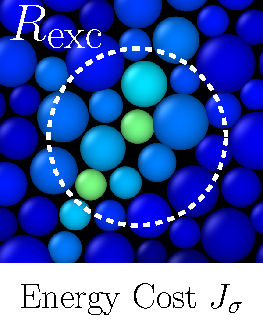
\includegraphics[height=0.3\textwidth]{slide_3/DF_Theory_Excitations_Zoom.pdf}}
\only<5->{\includegraphics[height=0.3\textwidth]{slide_5/Checkmark_exc.pdf}
}

} & \onslide<3->{
\only<3-4>{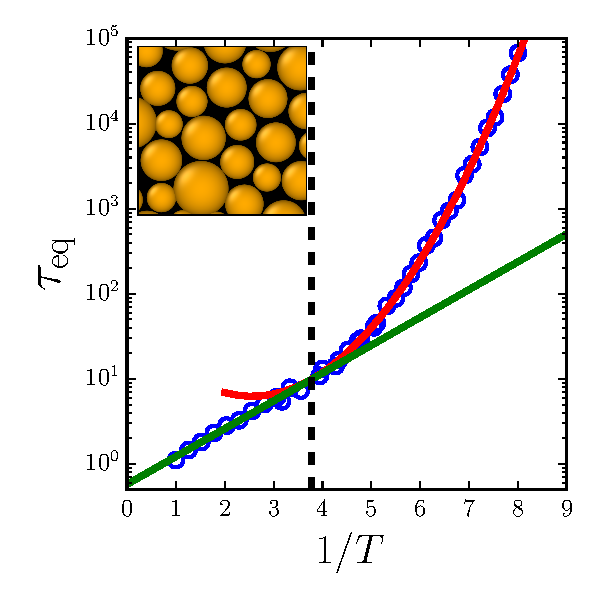
\includegraphics[height=0.3\textwidth]{slide_1/timerelax_poly12_4.pdf}
}
\only<5->{\includegraphics[height=0.3\textwidth]{slide_5/Checkmark_onset.pdf}}
} & \onslide<4->{\includegraphics[height=0.3\textwidth]{slide_3/facilitation_closer_2.pdf}} \\
\vspace{-1em}
\onslide<2->{
\only<2-4>{{\small What is the origin of "localized excitations" and their energy cost $\km{J_\sigma}$?}}
\only<5->{{\small  Hasyim, Mandadapu, \textit{J. Chem. Phys.} 155 (4), 44504 (2021)}}
} & 
\vspace{-1em}
\onslide<3->{
\only<2-4>{{\small Why do excitations emerge below an onset temperature $\km{T_\mathrm{o}}$?}}
\only<5->{{\small Fraggedakis, Hasyim, Mandadapu, \texttt{arXiv:2204.07528} (2022)}}
}
& 
\vspace{-1em}
\onslide<4->{{\small How does facilitation and $\km{\tilde{\gamma}}$ emerge from the glassy system?}} %\\
\end{tabulary}

\end{frame}




\begin{frame}\label{a.3}
\frametitle{Elastic Dynamical Facilitation (EDF) Theory: The Complete Picture}

EDF theory unifies elasticity with glassy dynamics through \textbf{three interconnected pillars} that provide a complete microscopic framework:

\vspace{0.5em}

\begin{columns}[T]
\begin{column}[T]{0.33\textwidth}

\centering\textbf{\Large Excitations}

\begin{figure}[t]
\centering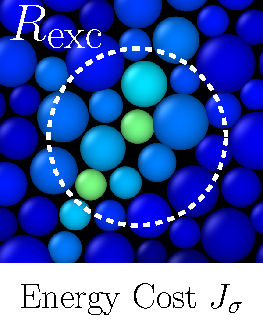
\includegraphics[height=0.45\textheight]{a.2-intro_dftheory/DF_Theory_Excitations_Zoom_2.pdf}
\caption{\textbf{Pure shear excitations} with energy scale $J_\sigma \sim G R_\mathrm{exc}^2 \epsilon_\mathrm{c}^2$}
\end{figure}

\end{column}

\begin{column}[T]{0.33\textwidth}

\centering\textbf{\Large Onset Temperature}

\begin{figure}[t]
\begin{center}
\centerline{\includegraphics[height=0.45\textheight]{c.1-kt_msdintro/msd-supercooledliq-5.pdf}}
\end{center}
\caption{\textbf{2D melting theory} explains $T_\mathrm{o}$ from elastic stability}
\end{figure}

\end{column}

\begin{column}[T]{0.33\textwidth}

\centering\textbf{\Large Facilitation}

\begin{figure}[t]
\begin{center}
\centerline{\includegraphics[height=0.45\textheight]{a.2-intro_dftheory/facilitation_closer_2.pdf}}
\end{center}
\caption{\textbf{Elastic stress fields} create emergent facilitation}
\end{figure}

\end{column}
\end{columns}

\vspace{1em}

\begin{block}{\centering Key Insight}
\centering \textbf{Elasticity} provides the microscopic foundation for all three pillars, creating a \textbf{unified quantitative theory}: 
$$\boxed{\text{EDF Theory} = \text{Elastic Excitations} + \text{Elastic Onset} + \text{Elastic Facilitation}}$$
\end{block}

\end{frame} 